\documentclass[11pt,twocolumn]{IEEEtran}

\usepackage[numbers]{natbib}
\usepackage{multicol}
\usepackage{xcolor}
\usepackage{listings}
\usepackage{xparse}
\usepackage{graphicx}
\usepackage{caption}

\graphicspath{{figures/}}

\NewDocumentCommand{\codeword}{v}{
	\texttt{\textcolor{blue}{#1}}
}

\renewcommand*{\bibfont}{\raggedright}

\setlength{\multicolsep}{6.0pt plus 2.0pt minus 1.5pt}

\title{DRAGONFIST}
\author{Joseph Boudreau, Andrew Ferrazzutti, Kia Shakiba, Zhongyu Zhao}
\date{December 9\textsuperscript{th}, 2018}

\begin{document}

	\maketitle

	\begin{abstract}
		The purpose of this paper is to examine the effects of applying transformations to images in the context of image classification neural networks.
		We investigate how using filtered images during training and inference affects the classification accuracy and resilience to adversarial attacks.
		The rationale supporting this methodology is that transforming the input images should obstruct or diffuse the intended perturbations of an adversarial example, while still preserving the significant features of the image so the model can effectively generalize and classify.
		Our findings indicate a marginal increase in both accuracy and a significant improvement in adversarial robustness for the ensemble model against black-box attacks and white-box attacks.
		Despite the improvement in accuracy, adversarial images are still misclassified $\>50\%$ of the time in most cases, so this model structure cannot be considered completely effective at this time.
	\end{abstract}

	\section{Introduction} \label{s:introduction}
In this paper we will describe and provide quantitative results for two model structures, each utilizing image filters in some way to create a more robust neural network.
The first structure is an ensemble model composed of several individually trained CNNs, each with a different image filter applied prior to classifying.
The outputs of every model are combined using a fitted logistic regression function.
The second design is a single CNN trained on a data set which has been augmented sets of filtered versions of each image in the original training data set.
During inference, the model will classify each filtered version of the image sequentially (having learned to classify different filtered versions of the images during training) and then similarly combine each prediction vector using logistic regression.
In both designs, we experiment with different combinations of filters in order to determine which are effective.
Our findings indicate a marginal increase in both accuracy (3-5\%) and a significant improvement in adversarial robustness (30-40\%) for the ensemble model against black-box attacks.
The second model design achieved less favorable results, exhibiting only marginal increases in performance and accuracy.
With regards to transformations, we investigate a multitude of existing filters, both linear and non-linear, in addition to implementing some custom filters and looking at their effectiveness.
Previous research indicates that median filters are effective at removing adversarial noise\cite{osadchy2016} - we found this to be the case in our experiments as well.
The most effective combination of filters to ensemble was Identity, Edge Detection, Min, Max, Rank, Median, and Gaussian.
In general, most filtered models exhibited small accuracy reductions compared to the same model trained with no filter.
The only filter which could achieve the same classification accuracy as an unfiltered model was a Sobel (edge detection) filter.
Extremely lossy filters performed, as expected, much worse on classification.
In general, we want to leverage the trade-off between distortion and accuracy in the ensemble to maximize resilience to adversarial perturbations.

For the purposes of convenience, as well as to limit the scope of variability in our research, every model in the ensemble shares the same underlying layer structure.
The models are implemented using the Keras Sequential interface and are composed of several 2D convolutional layers, a 2x2 max pooling layer, a final densely connected convolutional layer followd by an output Softmax activation function.
Unfortunately, due to a incompatibility between TensorFlow and the Cleverhans library, dropout regularization could not be utilized.

	\section{Motivation and Background} \label{s:motivationAndBackground}

	\section{Terminology} \label{s:terminology}
The name of the project, which encompasses the entire research scope of this work, is \“Dimensionally Reduced Adversarial Generations on Networks Filtered by Integrated Static Transformations\” which is shortened to Project DRAGONFIST.

Each model and filter combination is referred to as a "Classification Worker" (CLAW). The only parameters for CLAWs are the choice of filter as well as optional feature-wise preprocessing applied to the filtered dataset.

The ensembled model, composed of a set of CLAWs, is named the "Final Intuition Stage" (FIST). The model trained on the training set augmented with filtered versions of the training images is called the "Package Aggregate Learning Model" (PALM)
    \section{Image Filters} \label{s:filters}
	The proper selection of filters is important to the overall effectiveness of the algorithm. As previously mentioned, the intention of DRAGONFIST is to improve a machine learning model's resiliency against adversarial noise. Based on the work done by \citeauthor{goodfellow2015} \cite{goodfellow2015}, adversaries can target specific pixels in an image to which noise will be applied. As such, filters which combine the values of pixels with their neighbours are intuitively more desirable as they increase the difficulty of targeting specific areas of the image to which noise will be applied. Therefore, the following filters were considering when designing DRAGONFIST:
	\begin{multicols}{2}
		\begin{itemize}
			\item Edge detection
			\item Gaussian
			\item Average rows
			\item Average columns
			\item Rank
			\item Maximum
			\item Minimum
			\item Median
		\end{itemize}
	\end{multicols}

	\subsection{Descriptions} \label{s:filters:descriptions}
		In order to understand what the filters are doing to the images, a brief explanation of each is given.

		\subsubsection{Edge detection} \label{s:filters:descriptions:edgeDetection}
			The edge detection filter uses the Python library \codeword{skimage.filters.sobel} \cite{skikitImage}. This filter locates and isolates the edges of objects found in an image. An example of this filter applied to images in the MNIST Fashion database \cite{zalandoresearchFashionMNIST} can be seen in Appendix \ref{a:filters} Figure \ref{a:filters:edgeDetection}.

		\subsubsection{Gaussian} \label{s:filters:descriptions:gaussian}
			The Gaussian filter uses the Python library \codeword{skimage.filters.gaussian} \cite{skikitImage}. This filter convolves the image with a Gaussian function to create a ``blurring'' effect. An example of this filter applied to images in the MNIST Fashion database \cite{zalandoresearchFashionMNIST} can be seen in Appendix \ref{a:filters} Figure \ref{a:filters:gaussian}.

		\subsubsection{Average Rows} \label{s:filters:descriptions:averageRows}
			The average rows filter was created by us for this project. This filter finds the average pixel value (i.e. intensity for black and white images and RGB values for colour images) and sets all values in the row to the average. An example of this filter applied to images in the MNIST Fashion database \cite{zalandoresearchFashionMNIST} can be seen in Appendix \ref{a:filters} Figure \ref{a:filters:averageRows}.

		\subsubsection{Average Columns} \label{s:filters:descriptions:averageCols}
			The average columns filter was created by us for this project. This filter works similarly to the average rows filter described in Section \ref{s:filters:descriptions:averageRows} though is applied to an image's columns instead of rows. An example of this filter applied to images in the MNIST Fashion database \cite{zalandoresearchFashionMNIST} can be seen in Appendix \ref{a:filters} Figure \ref{a:filters:averageCols}.

		\subsubsection{Rank} \label{s:filters:descriptions:rank}
			The rank filter uses the Python library \codeword{scipy.ndimage.rank_filter} \cite{scipy}. This filter scans over an image with a rectangle (a 3x3 square was used in this project) and creates a histogram of the pixel values in the rectangle. One value in this histogram is then chosen to be applied to every pixel in the rectangle (a random value in the histogram was chosen for this project's rank filter). An example of this filter applied to images in the MNIST Fashion database \cite{zalandoresearchFashionMNIST} can be seen in Appendix \ref{a:filters} Figure \ref{a:filters:rank}.

			If the last value is chosen, a maximum filter is created. An example of this filter applied to images in the MNIST Fashion database \cite{zalandoresearchFashionMNIST} can be seen in Appendix \ref{a:filters} Figure \ref{a:filters:max}.

			If the first value is chosen, a minimum filter is created. An example of this filter applied to images in the MNIST Fashion database \cite{zalandoresearchFashionMNIST} can be seen in Appendix \ref{a:filters} Figure \ref{a:filters:min}.

			If the center value is chosen, a median filter is created. An example of this filter applied to images in the MNIST Fashion database \cite{zalandoresearchFashionMNIST} can be seen in Appendix \ref{a:filters} Figure \ref{a:filters:median}.

	\subsection{Filter accuracy} \label{s:filters:accuracy}
		When applying each filter to the system, it is important to remember the overall goal of the model -- to accurately classify its input. Therefore, each filter's accuracy in classification is important to consider to ensure the overall model maintains a high accuracy as well. Each filter was tested individually in order to determine its classification accuracy. The results of these tests can be observed in Table \ref{t:filterAccuracies}. All filters were trained using the same, standardized model architecture on the MNIST Fashion database \cite{zalandoresearchFashionMNIST} which contains \(60000\) images.

		Almost all filters demonstrated high accuracies except for the averaging filters. This was expected as these filters destroy much of the image's data which makes it harder to classify on the image later on; however, the filters were chosen to be included in the project as they combine a large amount of the image's pixels which intuitively makes it more difficult to target single pixels for adversarial noise.
		\begin{table}
			\begin{center}
				\caption{Image filter accuracies.}
				\label{t:filterAccuracies}
				\begin{tabular}{l|l}\hline
					\textbf{Filter} & \textbf{Accuracy (\(\%\))}\\\hline
					Identity & 91.57\\\hline
					Edge detection & 90.24\\\hline
					Gaussian & 90.07\\\hline
					Average rows & 79.66\\\hline
					Average columns & 82.09\\\hline
					Rank & 88.62\\\hline
					Maximum & 90.07\\\hline
					Minimum & 88.76\\\hline
					Median & 88.62\\\hline
				\end{tabular}
			\end{center}
		\end{table}

		These accuracies vary based on the number of epochs over which the model is trained. The accuracies of the mentioned filters for model over varying epochs can be seen in Figure \ref{f:filters:accuracies}.
		\begin{figure*}
			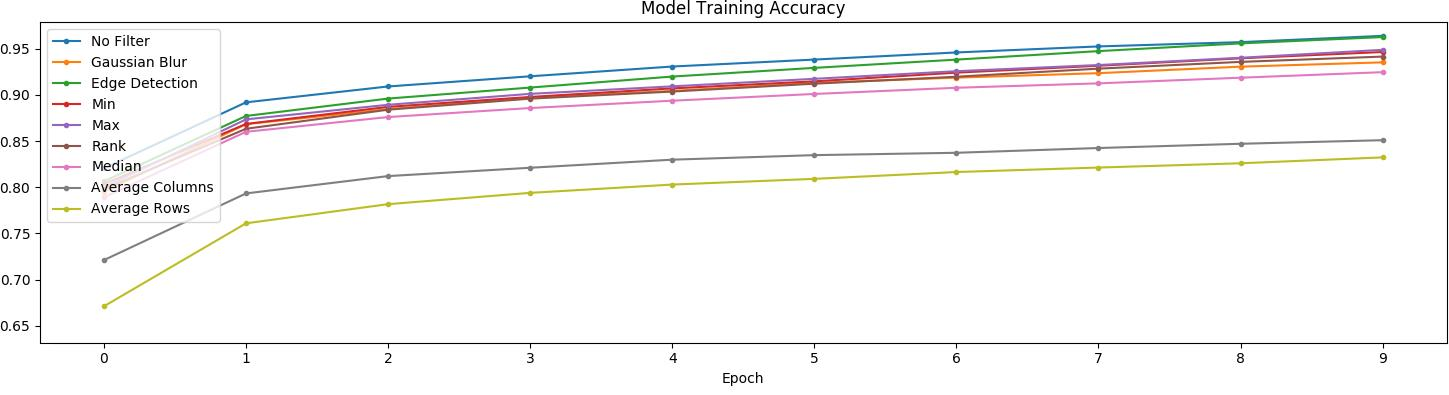
\includegraphics[width=\linewidth]{filter-accuracies.jpeg}
			\caption{Classification accuracy during training for various image filters.}
			\label{f:filters:accuracies}
		\end{figure*}

	\subsection{Filter selection} \label{s:filters:selection}
		As previously mentioned, filters were selected for use in the DRAGONFIST model based on their intuitive ability to combine data from neighbouring pixels in order to increase the difficulty of targetting specific pixels with adversarial noise. Due to time constraints, a more systematic approach to filter selection could not be created. As such, we leave this to potential future research. Tools which test a filter's ability to defend against adversarial noise could help identify filters which would improve DRAGONFIST's ability to mitigate attack would be extremely useful for this project.

	\section{White Box Attacks} \label{s:whiteboxattacks}
	\section{Black Box Attacks} \label{s:blackboxattacks}
Black-box attacks were implemented using a modified version of the attack provided by the Cleverhans library \cite{papernot2018cleverhans}.
The attack threat model assumes unlimited oracle ability on the target model, but no knowledge of the internal weights or biases of the model itself.
This threat model is arguably a more realistic and important scenario, compared to a model which assumes knowledge of the interior model.
This is because a model's structure should never be externally exposed and defense against these attacks can be mitigated by traditional security controls to prevent data theft and unwanted network access.
On the other hand, it is entirely valid for a model to expose query access publicly, either as part of an API or a GUI. Although true ``oracle'' access can be prevented with query limitations imposed on the user, there is still risk of gaining enough information from rate-limited access or of the controls being circumvented somehow.
Therefore, finding effective strategies for minimizing the effectiveness of black-box attacks are an important field of research in machine learning security.

The attack works by training a substitute CNN using the output labels of the target model in conjunction with the images given to the model to be classified.
This substitute model is a two layer CNN with ReLu activation functions and a Softmax normalization final layer.
This substitute model is then used to generate adversarial examples using the Fast Gradient Sign Method developed by \citeauthor{goodfellow2015} \cite{goodfellow2015}.
These adversarial examples are then tested against the original target model with the intention of misclassifying the input.
This attack utilizes the transferability characteristic of adversarial examples -- an adversarial image generated using one model will generally have a high probability of being misclassified by other models which perform the same classification task but may have been trained differently and use different internal structures.

We tested the effectiveness of both PALM and FIST model designs in increasing the classification accuracy of these transferred adversarial images, relative to a single ``standard'' model, as defined above.
The results of the black-box attack against the standard model for both the MNIST and CIFAR-10 datasets averaged over epochs ranging from 1 to 9 is given in Table \ref{t:standardBlackBoxAcc}.
\begin{table}
    \begin{center}
        \caption{Standard CNN Black-Box Accuracy}
        \label{t:standardBlackBoxAcc}
        \begin{tabular}{l|l|l}\hline
        \textbf{Dataset} & \textbf{Test Accuracy} & \textbf{Adversarial Accuracy}\\\hline
        MNIST & 90\% & 27\% \\\hline
        CIFAR-10 & 71\% & 24\% \\\hline
        \end{tabular}
    \end{center}
\end{table}

For the PALM, there was not a significant increase in classification accuracy on black-box adversarial examples.
The maximum adversarial accuracy achieved over a number of different trials with varying filter combinations was 14\% with a test accuracy of 87\% for the MNIST dataset, which represents a decrease compared to the average numbers for the standard model as seen in Table \ref{t:standardBlackBoxAcc}.

For the FIST, there were two ensembling implementations tested.
The first is a Logistic Regression function which was fitted to the output prediction vectors of each individual model in the ensemble.
The second was a simple averaging method of these prediction vectors.
The results of both ensembles over a range of training epochs and number of filters are shown in Tables \ref{t:logisticRegressionBlackBoxAcc} and \ref{t:basicAveragingBlackBoxAcc}.

\begin{table}
    \begin{center}
        \caption{Logistic Regression Ensemble Black-Box Accuracy}
        \label{t:logisticRegressionBlackBoxAcc}
        \begin{tabular}{l|l|l}\hline
        \textbf{\# Filters/Epochs} & \textbf{Test Accuracy} & \textbf{Adversarial Accuracy}\\\hline
        3/10 & 91\% & 33\% \\\hline
        6/3 & 89\% & 45\% \\\hline
        6/4 & 90\% & 39\% \\\hline
        6/5 & 89\% & 31\% \\\hline
        7/3 & 90\% & 48\% \\\hline
        8/3 & 87\% & 41\% \\\hline
        \end{tabular}
    \end{center}
\end{table}

\begin{table}
    \begin{center}
        \caption{Basic Averaging Ensemble Black-Box Accuracy}
        \label{t:basicAveragingBlackBoxAcc}
        \begin{tabular}{l|l|l}\hline
        \textbf{\# Filters/Epochs} & \textbf{Test Accuracy} & \textbf{Adversarial Accuracy}\\\hline
        4/4 & 91\% & 33\% \\\hline
        5/4 & 89\% & 49\% \\\hline
        5/5 & 91\% & 59\% \\\hline
        5/6 & 91\% & 53\% \\\hline
        5/7 & 91\% & 55\% \\\hline
        5/8 & 91\% & 41\% \\\hline
        6/5 & 90\% & 45\% \\\hline
        7/4 & 89\% & 50\% \\\hline
        7/5 & 91\% & 55\% \\\hline
        7/6 & 91\% & 51\% \\\hline
        7/7 & 89\% & 50\% \\\hline
        7/8 & 92\% & 43\% \\\hline
        \end{tabular}
    \end{center}
\end{table}

As can be seen in Tables \ref{t:logisticRegressionBlackBoxAcc} and \ref{t:basicAveragingBlackBoxAcc}, there was a significant improvement in both the test set accuracy as well as the adversarial accuracy when using the FIST ensembling model.
It is interesting to note that the basic averaging method outperformed the logistic regression function, although this may indicate that adversarial robustness is enhanced by accepting diversity and variance in the output response.
By weighting the individual CLAWS which do not classify as strongly as those which do, the FIST becomes more resilient to images which are outside the normal distribution and can handle these perturbed images better.
Out of all the FISTs tested, the best performing model was a basic averaging ensemble composed of 5 individual CLAWs trained for 5 epochs on images filtered by the following transformations:

\begin{itemize}
    \item Identity (No filter)
    \item Edge Detection w/ ZCA Whitening
    \item Rank
    \item Maximum
    \item Minimum
\end{itemize}

This FIST was able to increase the test accuracy from 90\% to 91\%, while also doubling the adversarial accuracy from 27\% to 59\%.
This is a noteworthy increase in model resilience against black-box attacks, especially since it required no additional training data or more complex model structure - simply an amalgamation of several models trained on images transformed using various filters.

	\section{Future Research} \label{s:futureresearch}
	\section{Conclusion} \label{s:conclusion}

	% ----- REFERENCES -----
	\bibliographystyle{IEEEtranN}
	\bibliography{references}{}

	%\pagebreak
	\appendix

\section{Appendix} \label{a}
	\subsection{Filtered Images} \label{a:filters}
		\begin{center}
			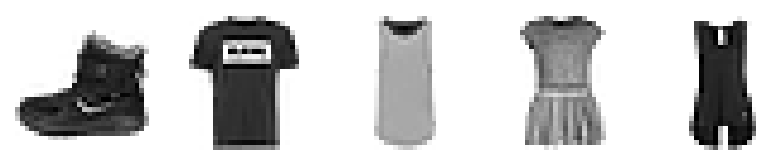
\includegraphics[width=\linewidth]{identity}
			\captionof{figure}{Unfiltered MNIST Fashion images.}
			\label{a:filters:identity}
		\end{center}

		\begin{center}
			
\includegraphics[width=\linewidth]{edge-detection}
			\captionof{figure}{Edge detection filter on MNIST Fashion images.}
			\label{a:filters:edgeDetection}
		\end{center}

		\begin{center}
			
\includegraphics[width=\linewidth]{gaussian}
			\captionof{figure}{Gaussian filter on MNIST Fashion images.}
			\label{a:filters:gaussian}
		\end{center}

		\begin{center}
			
\includegraphics[width=\linewidth]{average-rows}
			\captionof{figure}{Average rows filter on MNIST Fashion images.}
			\label{a:filters:averageRows}
		\end{center}

		\begin{center}
			
\includegraphics[width=\linewidth]{average-cols}
			\captionof{figure}{Average columns filter on MNIST Fashion images.}
			\label{a:filters:averageCols}
		\end{center}

		\begin{center}
			
\includegraphics[width=\linewidth]{rank}
			\captionof{figure}{Rank filter on MNIST Fashion images.}
			\label{a:filters:rank}
		\end{center}

		\begin{center}
			
\includegraphics[width=\linewidth]{max}
			\captionof{figure}{Maximum filter on MNIST Fashion images.}
			\label{a:filters:max}
		\end{center}

		\begin{center}
			
\includegraphics[width=\linewidth]{min}
			\captionof{figure}{Minimum filter on MNIST Fashion images.}
			\label{a:filters:min}
		\end{center}

		\begin{center}
			
\includegraphics[width=\linewidth]{median}
			\captionof{figure}{Median filter on MNIST Fashion images.}
			\label{a:filters:median}
		\end{center}


\end{document}
